
% \centering
%     % Input Image
%     \begin{minipage}{0.03\textwidth} % Narrow column for row label
%         \raggedleft
%         \rotatebox{90}{\text{Input Image}} % Vertical label for the first row
%     \end{minipage}
%     \begin{minipage}{0.12\textwidth}
%         \vspace{0.03cm}
%         \centering
%         
\includegraphics[width=\textwidth]{Collocated_Collage/input/frame344.png}
%     \end{minipage}
%     \begin{minipage}{0.12\textwidth}
%         \vspace{0.03cm}
%         \centering
%         
\includegraphics[width=\textwidth]{Collocated_Collage/input/frame44.png}
%     \end{minipage}
%     \begin{minipage}{0.12\textwidth}
%         \vspace{0.03cm}
%         \centering
%         
\includegraphics[width=\textwidth]{Collocated_Collage/input/frame129.png}
%     \end{minipage}
%     \begin{minipage}{0.12\textwidth}
%         \vspace{0.03cm}
%         \centering
%         
\includegraphics[width=\textwidth]{Collocated_Collage/10-20-vis/input/frame205.png}
%     \end{minipage}
%     \begin{minipage}{0.12\textwidth}
%         \vspace{0.03cm}
%         \centering
%         
\includegraphics[width=\textwidth]{Collocated_Collage/input/frame338.png}
%     \end{minipage}
%     \begin{minipage}{0.12\textwidth}
%         \vspace{0.03cm}
%         \centering
%         
\includegraphics[width=\textwidth]{Collocated_Collage/input/frame79.png}
%     \end{minipage}
%     \begin{minipage}{0.12\textwidth}
%         \vspace{0.03cm}
%         \centering
%         
\includegraphics[width=\textwidth]{Collocated_Collage/input/frame13.png}
%     \end{minipage}
%     \hspace{0.03\textwidth}
    


%     \begin{minipage}{0.03\textwidth} % Narrow column for row label
%         \raggedleft
%         \rotatebox{90}{\text{Ours}} % Vertical label for the first row
%     \end{minipage}
%       \begin{minipage}{0.12\textwidth}
%         \vspace{0.03cm}
%         \centering
%         
\includegraphics[width=\textwidth]{Collocated_Collage/output_bw_color/frame344.png}
%     \end{minipage}
%     \begin{minipage}{0.12\textwidth}
%         % \vspace{0.03cm}
%         \centering
%         
\includegraphics[width=\textwidth]{Collocated_Collage/output_bw_color/frame44.png}
%     \end{minipage}
%     \begin{minipage}{0.12\textwidth}
%         \vspace{0.03cm}
%         \centering
%         
\includegraphics[width=\textwidth]{Collocated_Collage/output_bw_color/frame129.png}
%     \end{minipage}
%     \begin{minipage}{0.12\textwidth}
%         \vspace{0.03cm}
%         \centering
%         
\includegraphics[width=\textwidth]{Collocated_Collage/10-20-vis/output/frame205.png}
%     \end{minipage}
%     \begin{minipage}{0.12\textwidth}
%         \vspace{0.03cm}
%         \centering
%         
\includegraphics[width=\textwidth]{Collocated_Collage/output_bw_color/frame338.png}
%     \end{minipage}
%     \begin{minipage}{0.12\textwidth}
%         \vspace{0.03cm}
%         \centering
%         
\includegraphics[width=\textwidth]{Collocated_Collage/output_bw_color/frame79.png}
%     \end{minipage}
%     \begin{minipage}{0.12\textwidth}
%         \vspace{0.03cm}
%         \centering
%         
\includegraphics[width=\textwidth]{Collocated_Collage/output_bw_color/frame13.png}
%     \end{minipage}
%     \hspace{0.03\textwidth}
    
%     \begin{minipage}{0.03\textwidth} % Narrow column for row label
%         \raggedleft
%         \rotatebox{90}{\text{Ground Truth}} % Vertical label for the first row
%       \end{minipage}
%       \begin{minipage}{0.12\textwidth}
%         \vspace{0.03cm}
%         \centering
%         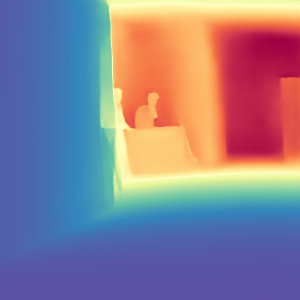
\includegraphics[width=\textwidth]{Collocated_Collage/gt_depth_color/frame344.png}
%     \end{minipage}
%     \begin{minipage}{0.12\textwidth}
%         % \vspace{0.03cm}
%         \centering
%         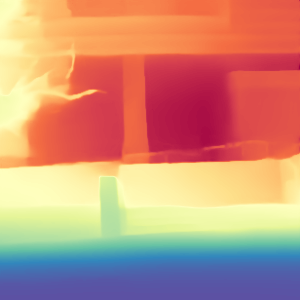
\includegraphics[width=\textwidth]{Collocated_Collage/gt_depth_color/frame44.png}
%     \end{minipage}
%     \begin{minipage}{0.12\textwidth}
%         \vspace{0.03cm}
%         \centering
%         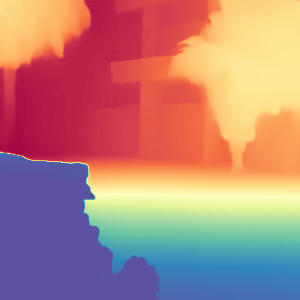
\includegraphics[width=\textwidth]{Collocated_Collage/gt_depth_color/frame129.png}
%     \end{minipage}
%     \begin{minipage}{0.12\textwidth}
%         \vspace{0.03cm}
%         \centering
%         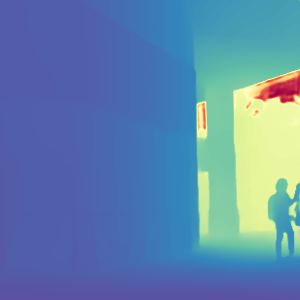
\includegraphics[width=\textwidth]{Collocated_Collage/10-20-vis/gt/frame205.png}
%     \end{minipage}
%     \begin{minipage}{0.12\textwidth}
%         \vspace{0.03cm}
%         \centering
%         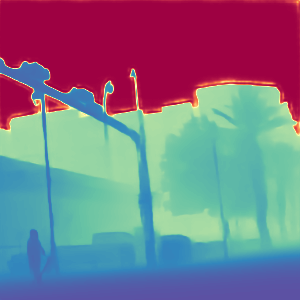
\includegraphics[width=\textwidth]{Collocated_Collage/gt_depth_color/frame338.png}
%     \end{minipage}
%     \begin{minipage}{0.12\textwidth}
%         \vspace{0.03cm}
%         \centering
%         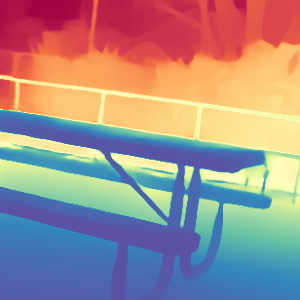
\includegraphics[width=\textwidth]{Collocated_Collage/gt_depth_color/frame79.png}
%     \end{minipage}
%     \begin{minipage}{0.12\textwidth}
%         \vspace{0.03cm}
%         \centering
%         
\includegraphics[width=\textwidth]{Collocated_Collage/gt_depth_color/frame13.png}
%     \end{minipage}
%     \hspace{0.03\textwidth}
%\vspace{-5mm}
    \centering
    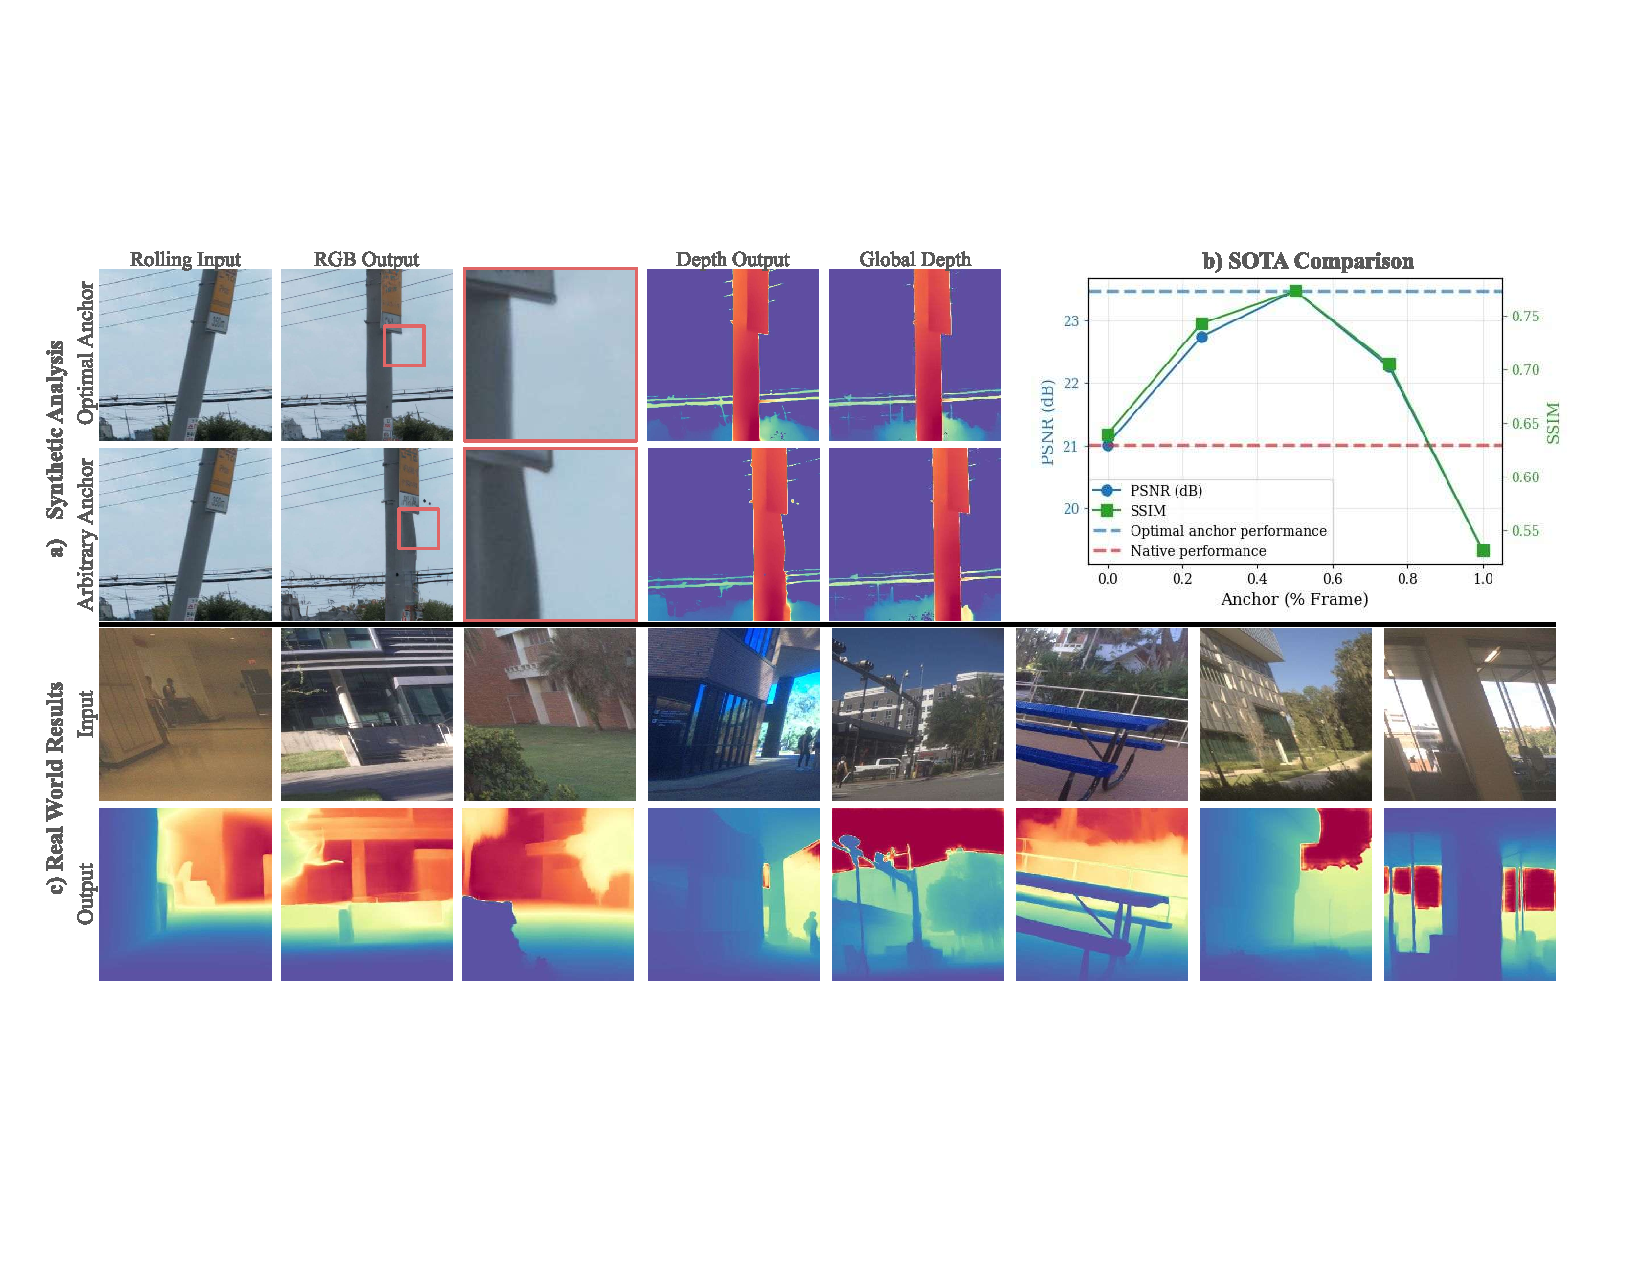
\includegraphics[width=0.95\linewidth,trim={.7cm 4.5cm 1cm 4.2cm},clip]{Figures/Rolling Shutter.pdf}%
    \vspace{-4mm}
    \captionof{figure}{
    \textbf{Anchor point formulation for rolling shutter correction}:
    \textbf{a)} We introduce the concept of an \emph{anchor point}, which defines the temporal reference used to align rolling shutter observations during correction.
    \textbf{b)} Quantitative analysis on a SOTA rolling shutter correction method~\cite{RS-Diffusion} shows that performance varies systematically with anchor-point selection, providing a significant metric boost around the proposed optimal anchor when compared to native implementation. This modification is \textbf{one line of code}, requiring no retraining of the model.
    \textbf{c)} We introduce visual foundation models to rolling shutter correction, providing geometrically consistent monocular depth from large rolling shutter distortions.
    }
    \label{fig:teaser_results}
